\section{Ejercicio 3}

\subsection{Descripci\'on del problema}

La entrada consta de un tablero de $n$ x $m$ casilleros y $k=n*m$ fichas cuadradas a colocar, estando cada uno de los 4 lados de las fichas identificado con un color. Se requiere colocar la mayor cantidad de fichas posibles en el tablero, tal que si 2 fichas son adyacentes, entonces el lado del cuadrado que tienen en com\'un tiene el mismo color. Las fichas ya vienen con una orientaci\'on y no pueden ser rotadas.
Ver la imagen \ref{ej_3:ej_1} para un ejemplo de la entrada, y la imagen \ref{ej_3:ej_1_sol} para ver una soluci\'on posible donde se colocan todas las fichas.
Se pide utilizar la t\'ecnica de \emph{Backtracking}
%\footnote{\emph{Backtracking} es una t\'ecnica para recorrer sistem\'aticamente todas las posibles configuraciones de un espacio asociado a soluciones candidatos de un problema computacional.}
y elaborar podas para mejorar los tiempos de ejecuci\'on.

\begin{figure}[!hbp]
\centering
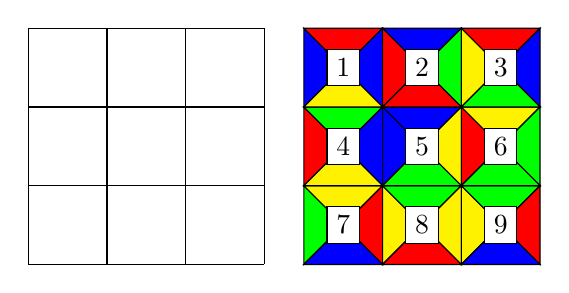
\begin{tikzpicture}
\draw (0,0) grid (3,3);

\draw[fill=green] (0 + 3.5, 0 + 0) -- (0 + 3.5, 0 + 1) -- (0 + 4, 0 + 0.5) -- cycle;
\draw[fill=yellow] (0 + 3.5, 0 + 1) -- (0 + 4.5, 0 + 1) -- (0 + 4, 0 + 0.5) -- cycle;
\draw[fill=red] (0 + 4.5, 0 + 1) -- (0 + 4.5, 0 + 0) -- (0 + 4, 0 + 0.5) -- cycle;
\draw[fill=blue] (0 + 3.5, 0 + 0) -- (0 + 4.5, 0 + 0) -- (0 + 4, 0 + 0.5) -- cycle;
\node[draw, fill=white] at (0 + 4, 0 + 0.5) {7};

\draw[fill=yellow] (1 + 3.5, 0 + 0) -- (1 + 3.5, 0 + 1) -- (1 + 4, 0 + 0.5) -- cycle;
\draw[fill=green] (1 + 3.5, 0 + 1) -- (1 + 4.5, 0 + 1) -- (1 + 4, 0 + 0.5) -- cycle;
\draw[fill=yellow] (1 + 4.5, 0 + 1) -- (1 + 4.5, 0 + 0) -- (1 + 4, 0 + 0.5) -- cycle;
\draw[fill=red] (1 + 3.5, 0 + 0) -- (1 + 4.5, 0 + 0) -- (1 + 4, 0 + 0.5) -- cycle;
\node[draw, fill=white] at (1 + 4, 0 + 0.5) {8};

\draw[fill=yellow] (2 + 3.5, 0 + 0) -- (2 + 3.5, 0 + 1) -- (2 + 4, 0 + 0.5) -- cycle;
\draw[fill=green] (2 + 3.5, 0 + 1) -- (2 + 4.5, 0 + 1) -- (2 + 4, 0 + 0.5) -- cycle;
\draw[fill=red] (2 + 4.5, 0 + 1) -- (2 + 4.5, 0 + 0) -- (2 + 4, 0 + 0.5) -- cycle;
\draw[fill=blue] (2 + 3.5, 0 + 0) -- (2 + 4.5, 0 + 0) -- (2 + 4, 0 + 0.5) -- cycle;
\node[draw, fill=white] at (2 + 4, 0 + 0.5) {9};

\draw[fill=red] (0 + 3.5, 1 + 0) -- (0 + 3.5, 1 + 1) -- (0 + 4, 1 + 0.5) -- cycle;
\draw[fill=green] (0 + 3.5, 1 + 1) -- (0 + 4.5, 1 + 1) -- (0 + 4, 1 + 0.5) -- cycle;
\draw[fill=blue] (0 + 4.5, 1 + 1) -- (0 + 4.5, 1 + 0) -- (0 + 4, 1 + 0.5) -- cycle;
\draw[fill=yellow] (0 + 3.5, 1 + 0) -- (0 + 4.5, 1 + 0) -- (0 + 4, 1 + 0.5) -- cycle;
\node[draw, fill=white] at (0 + 4, 1 + 0.5) {4};

\draw[fill=blue] (1 + 3.5, 1 + 0) -- (1 + 3.5, 1 + 1) -- (1 + 4, 1 + 0.5) -- cycle;
\draw[fill=blue] (1 + 3.5, 1 + 1) -- (1 + 4.5, 1 + 1) -- (1 + 4, 1 + 0.5) -- cycle;
\draw[fill=yellow] (1 + 4.5, 1 + 1) -- (1 + 4.5, 1 + 0) -- (1 + 4, 1 + 0.5) -- cycle;
\draw[fill=green] (1 + 3.5, 1 + 0) -- (1 + 4.5, 1 + 0) -- (1 + 4, 1 + 0.5) -- cycle;
\node[draw, fill=white] at (1 + 4, 1 + 0.5) {5};

\draw[fill=red] (2 + 3.5, 1 + 0) -- (2 + 3.5, 1 + 1) -- (2 + 4, 1 + 0.5) -- cycle;
\draw[fill=yellow] (2 + 3.5, 1 + 1) -- (2 + 4.5, 1 + 1) -- (2 + 4, 1 + 0.5) -- cycle;
\draw[fill=green] (2 + 4.5, 1 + 1) -- (2 + 4.5, 1 + 0) -- (2 + 4, 1 + 0.5) -- cycle;
\draw[fill=green] (2 + 3.5, 1 + 0) -- (2 + 4.5, 1 + 0) -- (2 + 4, 1 + 0.5) -- cycle;
\node[draw, fill=white] at (2 + 4, 1 + 0.5) {6};

\draw[fill=blue] (0 + 3.5, 2 + 0) -- (0 + 3.5, 2 + 1) -- (0 + 4, 2 + 0.5) -- cycle;
\draw[fill=red] (0 + 3.5, 2 + 1) -- (0 + 4.5, 2 + 1) -- (0 + 4, 2 + 0.5) -- cycle;
\draw[fill=blue] (0 + 4.5, 2 + 1) -- (0 + 4.5, 2 + 0) -- (0 + 4, 2 + 0.5) -- cycle;
\draw[fill=yellow] (0 + 3.5, 2 + 0) -- (0 + 4.5, 2 + 0) -- (0 + 4, 2 + 0.5) -- cycle;
\node[draw, fill=white] at (0 + 4, 2 + 0.5) {1};

\draw[fill=red] (1 + 3.5, 2 + 0) -- (1 + 3.5, 2 + 1) -- (1 + 4, 2 + 0.5) -- cycle;
\draw[fill=blue] (1 + 3.5, 2 + 1) -- (1 + 4.5, 2 + 1) -- (1 + 4, 2 + 0.5) -- cycle;
\draw[fill=green] (1 + 4.5, 2 + 1) -- (1 + 4.5, 2 + 0) -- (1 + 4, 2 + 0.5) -- cycle;
\draw[fill=red] (1 + 3.5, 2 + 0) -- (1 + 4.5, 2 + 0) -- (1 + 4, 2 + 0.5) -- cycle;
\node[draw, fill=white] at (1 + 4, 2 + 0.5) {2};

\draw[fill=yellow] (2 + 3.5, 2 + 0) -- (2 + 3.5, 2 + 1) -- (2 + 4, 2 + 0.5) -- cycle;
\draw[fill=red] (2 + 3.5, 2 + 1) -- (2 + 4.5, 2 + 1) -- (2 + 4, 2 + 0.5) -- cycle;
\draw[fill=blue] (2 + 4.5, 2 + 1) -- (2 + 4.5, 2 + 0) -- (2 + 4, 2 + 0.5) -- cycle;
\draw[fill=green] (2 + 3.5, 2 + 0) -- (2 + 4.5, 2 + 0) -- (2 + 4, 2 + 0.5) -- cycle;
\node[draw, fill=white] at (2 + 4, 2 + 0.5) {3};

\end{tikzpicture}
\caption{Un tablero de 3 x 3 con las fichas que se deben colocar en el tablero}
\label{ej_3:ej_1}
\end{figure}

\begin{figure}[!hbp]
\centering
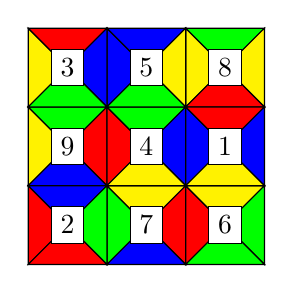
\begin{tikzpicture}

\draw[fill=green] (1 + 0, 0 + 0) -- (1 + 0, 0 + 1) -- (1 + 0.5, 0 + 0.5) -- cycle;
\draw[fill=yellow] (1 + 0, 0 + 1) -- (1 + 1, 0 + 1) -- (1 + 0.5, 0 + 0.5) -- cycle;
\draw[fill=red] (1 + 1, 0 + 1) -- (1 + 1, 0 + 0) -- (1 + 0.5, 0 + 0.5) -- cycle;
\draw[fill=blue] (1 + 0, 0 + 0) -- (1 + 1, 0 + 0) -- (1 + 0.5, 0 + 0.5) -- cycle;
\node[draw, fill=white] at (1 + 0.5, 0 + 0.5) {7};

\draw[fill=yellow] (2 + 0, 2 + 0) -- (2 + 0, 2 + 1) -- (2 + 0.5, 2 + 0.5) -- cycle;
\draw[fill=green] (2 + 0, 2 + 1) -- (2 + 1, 2 + 1) -- (2 + 0.5, 2 + 0.5) -- cycle;
\draw[fill=yellow] (2 + 1, 2 + 1) -- (2 + 1, 2 + 0) -- (2 + 0.5, 2 + 0.5) -- cycle;
\draw[fill=red] (2 + 0, 2 + 0) -- (2 + 1, 2 + 0) -- (2 + 0.5, 2 + 0.5) -- cycle;
\node[draw, fill=white] at (2 + 0.5, 2 + 0.5) {8};

\draw[fill=yellow] (0 + 0, 1 + 0) -- (0 + 0, 1 + 1) -- (0 + 0.5, 1 + 0.5) -- cycle;
\draw[fill=green] (0 + 0, 1 + 1) -- (0 + 1, 1 + 1) -- (0 + 0.5, 1 + 0.5) -- cycle;
\draw[fill=red] (0 + 1, 1 + 1) -- (0 + 1, 1 + 0) -- (0 + 0.5, 1 + 0.5) -- cycle;
\draw[fill=blue] (0 + 0, 1 + 0) -- (0 + 1, 1 + 0) -- (0 + 0.5, 1 + 0.5) -- cycle;
\node[draw, fill=white] at (0 + 0.5, 1 + 0.5) {9};

\draw[fill=red] (1 + 0, 1 + 0) -- (1 + 0, 1 + 1) -- (1 + 0.5, 1 + 0.5) -- cycle;
\draw[fill=green] (1 + 0, 1 + 1) -- (1 + 1, 1 + 1) -- (1 + 0.5, 1 + 0.5) -- cycle;
\draw[fill=blue] (1 + 1, 1 + 1) -- (1 + 1, 1 + 0) -- (1 + 0.5, 1 + 0.5) -- cycle;
\draw[fill=yellow] (1 + 0, 1 + 0) -- (1 + 1, 1 + 0) -- (1 + 0.5, 1 + 0.5) -- cycle;
\node[draw, fill=white] at (1 + 0.5, 1 + 0.5) {4};

\draw[fill=blue] (1 + 0, 2 + 0) -- (1 + 0, 2 + 1) -- (1 + 0.5, 2 + 0.5) -- cycle;
\draw[fill=blue] (1 + 0, 2 + 1) -- (1 + 1, 2 + 1) -- (1 + 0.5, 2 + 0.5) -- cycle;
\draw[fill=yellow] (1 + 1, 2 + 1) -- (1 + 1, 2 + 0) -- (1 + 0.5, 2 + 0.5) -- cycle;
\draw[fill=green] (1 + 0, 2 + 0) -- (1 + 1, 2 + 0) -- (1 + 0.5, 2 + 0.5) -- cycle;
\node[draw, fill=white] at (1 + 0.5, 2 + 0.5) {5};

\draw[fill=red] (2 + 0, 0 + 0) -- (2 + 0, 0 + 1) -- (2 + 0.5, 0 + 0.5) -- cycle;
\draw[fill=yellow] (2 + 0, 0 + 1) -- (2 + 1, 0 + 1) -- (2 + 0.5, 0 + 0.5) -- cycle;
\draw[fill=green] (2 + 1, 0 + 1) -- (2 + 1, 0 + 0) -- (2 + 0.5, 0 + 0.5) -- cycle;
\draw[fill=green] (2 + 0, 0 + 0) -- (2 + 1, 0 + 0) -- (2 + 0.5, 0 + 0.5) -- cycle;
\node[draw, fill=white] at (2 + 0.5, 0 + 0.5) {6};

\draw[fill=blue] (2 + 0, 1 + 0) -- (2 + 0, 1 + 1) -- (2 + 0.5, 1 + 0.5) -- cycle;
\draw[fill=red] (2 + 0, 1 + 1) -- (2 + 1, 1 + 1) -- (2 + 0.5, 1 + 0.5) -- cycle;
\draw[fill=blue] (2 + 1, 1 + 1) -- (2 + 1, 1 + 0) -- (2 + 0.5, 1 + 0.5) -- cycle;
\draw[fill=yellow] (2 + 0, 1 + 0) -- (2 + 1, 1 + 0) -- (2 + 0.5, 1 + 0.5) -- cycle;
\node[draw, fill=white] at (2 + 0.5, 1 + 0.5) {1};

\draw[fill=red] (0 + 0, 0 + 0) -- (0 + 0, 0 + 1) -- (0 + 0.5, 0 + 0.5) -- cycle;
\draw[fill=blue] (0 + 0, 0 + 1) -- (0 + 1, 0 + 1) -- (0 + 0.5, 0 + 0.5) -- cycle;
\draw[fill=green] (0 + 1, 0 + 1) -- (0 + 1, 0 + 0) -- (0 + 0.5, 0 + 0.5) -- cycle;
\draw[fill=red] (0 + 0, 0 + 0) -- (0 + 1, 0 + 0) -- (0 + 0.5, 0 + 0.5) -- cycle;
\node[draw, fill=white] at (0 + 0.5, 0 + 0.5) {2};

\draw[fill=yellow] (0 + 0, 2 + 0) -- (0 + 0, 2 + 1) -- (0 + 0.5, 2 + 0.5) -- cycle;
\draw[fill=red] (0 + 0, 2 + 1) -- (0 + 1, 2 + 1) -- (0 + 0.5, 2 + 0.5) -- cycle;
\draw[fill=blue] (0 + 1, 2 + 1) -- (0 + 1, 2 + 0) -- (0 + 0.5, 2 + 0.5) -- cycle;
\draw[fill=green] (0 + 0, 2 + 0) -- (0 + 1, 2 + 0) -- (0 + 0.5, 2 + 0.5) -- cycle;
\node[draw, fill=white] at (0 + 0.5, 2 + 0.5) {3};

\end{tikzpicture}
\caption{Soluci\'on colocando todas las fichas del problema de la figura \ref{ej_3:ej_1}}
\label{ej_3:ej_1_sol}
\end{figure}



\subsection{Ideas para la resoluci\'on} \label{ej_3:idea}

Como los casilleros del tablero pueden quedar vac\'ios si no se encuentra una ficha que pueda ser colocada,
llamando $k=n*m$, $n$ y $m$ las filas y columnas del tablero, y $i$ a la cantidad de casilleros que se dejan vac\'ios, para cada $i$ se pueden elegir de $\binom{k}{i}$ formas diferentes esos $i$ casilleros a dejar vac\'ios (porque de la cantidad de casilleros totales, se eligen $i$ los cuales son indistinguibles),
y para cada $i$, nos quedan $k - i$ casilleros donde colocar fichas, las cuales s\'i son distinguibles, y se pueden colocar de $k!/i!$ formas diferentes.
Por lo tanto, la cantidad de combinaciones que se pueden hacer con el tablero incluyendo dejar casilleros libres, es (\ref{ej_3:combinaciones})
\begin{equation}
	\sum_{i=0}^{k}\binom{k}{i}\frac{k!}{i!} \label{ej_3:combinaciones}
\end{equation}
\begin{equation*}
\begin{split}
	= \sum_{i=0}^{k}\frac{k!}{i!(k-i)!}\frac{k!}{i!}\\
	= \sum_{i=0}^{k}\frac{(k!)^2}{(i!)^2(k-i)!} \\
	= (k!)^2\sum_{i=0}^{k}\frac{1}{(i!)^2(k-i)!}
\end{split}
\end{equation*}

Pero para la resoluci\'on del problema s\'olo nos interesan las combinaciones v\'alidas, la idea que se plantea es ir completando el tablero casillero a casillero, y en cada casillero intentar colocar todas las fichas tal que no hayan sido colocadas antes y que al colocarla siga siendo una combinaci\'on v\'alida (que coincidan los colores con las fichas adyacentes). As\'i se van analizando s\'olo las combinaciones v\'alidas, que ser\'an menor o igual que la cuenta anterior (\ref{ej_3:k}), y retornando la combinaci\'on que contenga la mayor cantidad de fichas colocadas.

Como el resultado ser\'a una s\'ola combinaci\'on que contenga la mayor cantdidad de fichas colocadas, se puede elaborar una \emph{poda} para descartar combinaciones a medida que se est\'an armando para no terminar de generarlas y analizarlas si se determina que aunque se sigan agregando fichas a la combinaci\'on en la que se est\'a trabajando, no podr\'a contener m\'as fichas colocadas que alguna otra combinaci\'on que ya se haya calculado.
Supongamos que se est\'a trabajando con un tablero de 3 x 3 (9 fichas), y ya se proces\'o una combinaci\'on que s\'olo se deja vac\'io un casillero (contiene 8 fichas colocadas), guardando esta posible soluci\'on como la que m\'as fichas contiene; y actualmente se est\'a procesando una posible soluci\'on que ya analiz\'o 6 casilleros del tablero (quedando 3 a\'un por procesar), pero tuvo que dejar 2 casilleros vac\'ios (es decir, de los 6 casilleros 4 contienen fichas),
si en los 3 casilleros restantes colocase 3 fichas (lo m\'aximo que puede conseguir), esta combinaci\'on tendr\'ia 7 fichas colocadas (4 que ya hab\'ia colocado mas 3 posibles fichas que puede colocar a continuaci\'on) y 2 casilleros vac\'ios, siendo menor a la candidad de 8 fichas de la soluci\'on guardad como m\'axima encontrada hasta el momento, por lo que se puede descartar la soluci\'on que se ven\'ia procesando porque nunca podr\'ia llegar a ser una soluci\'on al problema.

\subsubsection{Algoritmo para la resoluci\'on propuesta} \label{ej_3:algo}

Como se describi\'o en la secci\'on (\ref{ej_3:idea}), la resoluci\'on del problema se basa en 2 ideas, s\'olo analizar combinaciones v\'alidas y descartar combinaciones si ya se calcula que no pueden superar a una combinaci\'on m\'axima ya encontrada.
Se propone el algoritmo \ref{ej_3:pseudo}.

\begin{algorithm}
	\caption{maximizarTablero} \label{ej_3:pseudo}
\end{algorithm} %sino no divide el codigo en paginas
\begin{algorithmic}[1]
	\Require \emph{tablero}: el tablero donde se ir\'an colocando las fichas
	\Require \emph{n, m}: filas y columnas del tablero
	\Require \emph{fichas\_disponibles}: array con las fichas aun diponibles por poner
	\Require \emph{i\_actual, j\_actual}: la posici\'on que se tiene que procesar
	\Require \emph{casilleros\_calculados}: cantidad de casilleros que ya se procesaron
	\Require \emph{fichas\_colocadas}: cantidad de fichas colocadas (no se cuentan los casilleros vac\'ios dejados)
	\Require \emph{tablero\_optimo}: el optimo encontrado hasta el momento
	\Require \emph{fichas\_maximas}: cantidad m\'axima de fichas que se pudieron colocar en el tablero\_optimo
	\Ensure La funci\'on va a dejar en \emph{tablero\_optimo} y en \emph{fichas\_maximas} la mejor combinaci\'on que pudo encontrar de fichas tal que las fichas adyacentes comparten el color en el borde que tienen en com\'un, y es la combinaci\'on en la que m\'as fichas se pudo colocar
	\Statex
	\Procedure{maximizarTablero}{tablero, n, m, fichas\_disponibles, i\_actual, j\_actual, casilleros\_calculados, fichas\_colocadas, tablero\_optimo, fichas\_maximas}
	\State $total\_casilleros \gets n*m$
	\State $n\_fichas \gets total\_casilleros$
	\If{$casilleros\_calculados = total\_casilleros$} \label{ej_3:pseudo:base}
		\If{$fichas\_colocadas > fichas\_maximas$}
			\State copiarTablero(tablero\_optimo, tablero)
			\State $fichas\_maximas \gets fichas\_colocadas$
		\EndIf
		\State return
	\EndIf \label{ej_3:pseudo:base_end}
	\If{$total\_casilleros - casilleros\_calculados + fichas\_colocadas <= fichas\_maxima$} \label{ej_3:pseudo:poda}
		\State return
	\EndIf
	\State $proximo\_i \gets i\_actual$ \label{ej_3:pseudo:proximo}
	\State $proximo\_j \gets j\_actual$
	\If{$i\_actual = n - 1$}
		\State $proximo\_i \gets 0$
		\State $proximo\_j++$
	\Else
		\State $proximo\_i++$
	\EndIf \label{ej_3:pseudo:proximo_end}
	\For{$f \in fichas\_disponibles$} \label{ej_3:pseudo:fichas} \label{ej_3:pseudo:disponible}
		\If{validaColocar(f, tablero, i\_actual, j\_actual)} \label{ej_3:pseudo:valida}
			\State $tablero[i\_actual][j\_actual] = f$ \label{ej_3:pseudo:coloca}
			\If{$\neg f->vacia$} \label{ej_3:pseudo:vacia}
				\State $fichas\_nuevas \gets fichas\_disponibles - f$
				\State $fichas\_colocadas++$
			\Else
				\State $fichas\_nuevas \gets fichas\_disponibles$
			\EndIf
			\State maximizarTablero(tablero, n, m, fichas\_nuevas, i\_proximo, j\_proximo, casilleros\_calculados + 1, fichas\_colocadas, tablero\_optimo, fichas\_maximas) \label{ej_3:pseudo:recursion}
			\If{$\neg f->vacia$}
				\State $fichas\_colocadas--$
			\EndIf
		\EndIf
	\EndFor \label{ej_3:pseudo:fichas_end}
	\EndProcedure
	\Statex
	\Procedure{bool validaColocar}{ficha, tablero, i, j} \label{ej_3:pseudo:validaColocar}
		\If{$ficha->vacia$}
			\State $return \gets true$
		\EndIf
		\If{$j > 0$}
			\If{$\neg tablero[i][j - 1]->vacia$}
				\If{$tablero[i][j - 1]->derecha \neq fichas->izquierda$}
					\State $return \gets false$
				\EndIf
			\EndIf
		\EndIf
		\If{$i > 0$}
			\If{$\neg tablero[i - 1][j]->vacia$}
				\If{$tablero[i- 1][j]->abajo \neq fichas->arriba$}
					\State $return \gets false$
				\EndIf
			\EndIf
		\EndIf
		\State $return \gets true$
	\EndProcedure
\end{algorithmic}

%\begin{procedure}
%	\SetKwProg{Fn}{}{}{}
%	\SetStartEndCondition{ (}{)}{)}\SetAlgoBlockMarkers{\{}{\}}
%	\SetKwFunction{maximizarTablero}{maximizarTablero}
%	\SetKwFunction{copiarTablero}{copiarTablero}
%	\KwIn{\emph{tablero}: el tablero donde se ir\'an colocando las fichas}
%	\KwIn{\emph{n, m}: filas y columnas del tablero}
%	\KwIn{\emph{fichas\_disponibles}: array con las fichas aun diponibles por poner}
%	\KwIn{\emph{i\_actual, j\_actual}: la posici\'on que se tiene que procesar}
%	\KwIn{\emph{casilleros\_calculados}: cantidad de casilleros que ya se procesaron}
%	\KwIn{\emph{fichas\_colocadas}: cantidad de fichas colocadas (no se cuentan los casilleros vac\'ios dejados)}
%	\KwIn{\emph{tablero\_optimo}: el optimo encontrado hasta el momento}
%	\KwIn{\emph{fichas\_maximas}: cantidad m\'axima de fichas que se pudieron colocar en el tablero\_optimo}
%	\KwOut{La funci\'on va a dejar en \emph{tablero\_optimo} y en \emph{fichas\_maximas} la mejor combinaci\'on que pudo encontrar de fichas tal que las fichas adyacentes comparten el color en el borde que tienen en com\'un, y es la combinaci\'on en la que m\'as fichas se pudo colocar}
%	\Fn(){void \maximizarTablero{tablero, n, m, fichas\_disponibles, i\_actual, j\_actual, casilleros\_calculados, fichas\_colocadas, tablero\_optimo, fichas\_maximas}}{
%		$total\_casilleros \leftarrow n*m$\;
%		$n\_fichas \leftarrow total\_casilleros$\;
%		\If{$casilleros\_calculados = total\_casilleros$}{
%			\If{$fichas\_colocadas > fichas\_maximas$}{
%				\copiarTablero{tablero\_optimo, tablero}
%				$fichas\_maximas \leftarrow fichas\_colocadas$\;
%			}
%			\KwRet
%		}
%		\If{$total\_casilleros - casilleros\_calculados + fichas\_colocadas <= fichas\_maxima$}{
%			\KwRet;
%		}
%		$proximo\_i \leftarrow i\_actual$\;
%		$proximo\_j \leftarrow j\_actual$\;
%		\uIf{$j\_actual = m - 1$}{
%			$proximo\_j = 0$\;
%			$proximo\_i++$\;
%		}
%		\Else{
%			$proximo\_j++$\;
%		}
%		\For{$i \leftarrow 0; i < n\_fichas; i++$}{
%			\If{$fichas\_disponibles[i]$}{
%				\If{$fichas\_disponibles[i]->numero >= 0$}{
%					\If{$j\_actual > 0$}{
%						\If{$tablero[i\_actual][j\_actual - 1]->numero >= 0$}{
%							\If{$tablero[i\_actual][j\_actual - 1]->derecha \neq fichas\_disponibles[i]->izquierda$}{
%								$continue$\;
%							}
%						}
%					}
%					\If{$i\_actual > 0$}{
%						\If{$tablero[i\_actual - 1][j\_actual]->numero >= 0$}{
%							\If{$tablero[i\_actual - 1][j\_actual]->abajo \neq fichas\_disponibles[i]->arriba$}{
%								$continue$\;
%							}
%						}
%					}
%				}
%				$tablero[i\_actual][j\_actual] = fichas\_disponibles[i]$\;
%				\If{$fichas\_disponibles[i]->numero >= 0$}{
%					$fichas\_disponibles[i] \leftarrow NULL$\;
%					$fichas\_en\_tablero++$\;
%				}
%				$casilleros\_tablero++$\;
%				\maximizarTablero{tablero, n, m, fichas\_disponibles, i\_proximo, j\_proximo, casilleros\_calculados, fichas\_colocadas, tablero\_optimo, fichas\_maximas}
%				\If{$fichas[i].numero >= 0$}{
%					$fichas\_disponibles[i] \leftarrow \&fichas[i]$\;
%					$fichas\_en\_tablero--$\;
%				}
%				$casilleros\_tablero--$\;
%			}
%		}
%		\KwRet
%	}
%	\caption{maximizarTablero()} \label{ej_3:pseudo}
%\end{procedure}



La funci\'on maximizarTablero (algoritmo \ref{ej_3:pseudo}), es recursiva y en la primera llamada debe llamarse con \emph{tablero}, siendo una matriz de $n * m$, donde se colocar\'an las fichas.
\emph{n} y \emph{m} son las filas y columnas del \emph{tablero}.
\emph{fichas\_disponibles} tiene que contener todas las fichas que vinieron en la entrada y con el campo \emph{vac\'ia} en $false$, m\'as una ficha con el campo \emph{vac\'ia} en $true$ (para indicar que ese casillero se dejo vac\'io).
\emph{i\_actual}, \emph{j\_actual}, \emph{casilleros\_calculados} y \emph{fichas\_colocadas} tienen que estar en $0$.
\emph{tablero\_optimo} es donde se va a colocar el tablero con mayor cantidad de fichas colocadas, y en \emph{fichas\_maximas} se va a colocar la cantidad de fichas en dicho tablero, \emph{fichas\_maximas} debe estar en un valor menor a 0 cuando se llama al algoritmo.

El algoritmo (\ref{ej_3:pseudo}) lo que realiza es llamarse recursivamente probando en cada casillero todas las fichas que esten disponibles para poner y que sea valido colocarlas.

Entre las l\'ineas \ref{ej_3:pseudo:base} y \ref{ej_3:pseudo:base_end} se encuentra el caso base de la recursi\'on, el cual sucede cuando ya se procesaron todos los casilleros, si la cantidad de fichas colocadas es mayor a la cantidad m\'axima que se hab\'ia almacenado, entonces reemplaza el \emph{tablero\_optimo} con el tablero actual, y actualiza la variable \emph{fichas\_maximas}.

Luego en la l\'inea \ref{ej_3:pseudo:poda} se encuentra la \emph{poda} para cortar con la recursi\'on antes de procesar todos los casilleros si aunque se completen todos los casilleros restantes con fichas, no superar\'an la cantidad m\'axima de fichas que ya se almacen\'o con otra combinaci\'on.

Entre las l\'ineas \ref{ej_3:pseudo:proximo} y \ref{ej_3:pseudo:proximo_end} se calcula el pr\'oximo casillero que se deber\'a llamar en la recursi\'on

Y por \'ultimo entre las l\'ineas \ref{ej_3:pseudo:fichas} y \ref{ej_3:pseudo:fichas_end} se buscan todas las fichas disponibles para colocar (l\'inea \ref{ej_3:pseudo:disponible}) y que sea v\'alida su colocaci\'on (l\'inea \ref{ej_3:pseudo:valida}), entonces si se cumplen dichas condiciones,
coloca la ficha en el tablero (l\'inea \ref{ej_3:pseudo:coloca}) y si no es la ficha que corresponde al casillero vac\'io (l\'inea \ref{ej_3:pseudo:vacia}) la elmina de las fichas disponibles,
y se llama recursivamente (l\'linea \ref{ej_3:pseudo:recursion}) con la nueva posici\'on a analizar.

Tambi\'em se encuentra la funci\'on \emph{validaColocar} como una funci\'on auxiliar que retornar\'a $true$ si colocar la \emph{ficha} en el \emph{tablero} en la posici\'on \emph{i, j},
pero tiene en cuenta que el tablero se va completando de izquierda a derecha y de abajo a izquierda (el $(0; 0)$ corresponde a arriba a la izquierda), y en base a esto s\'olo chequea 2 lados de la ficha a colocar y no los 4.

En la secci\'on (\ref{ej_3:justificacion}) se hablar\'a sobre la justificaci\'on y correctitud del algoritmo.

Se puede ver una implementaci\'on del algoritmo en la secci\'on \ref{codigo_2}.

\subsubsection{Ejemplo de la resoluci\'on propuesta}
\label{ej_3:ejemplo}

Siguiendo los pasos del algoritmo de la secci\'on \ref{ej_3:algo}, se procede a un ejemplo de la ejecuci\'on con un tablero de 2 x 2 y 4 fichas, y 3 colores (imagen \ref{ej_3:entrada}, todas las im\'agenes se encuentran al final de la secci\'on \ref{ej_3:ejemplo}), agregando la ficha \emph{V} para indicar dejar el casillero vac\'io

El algoritmo comienza en la posici\'on $(0;0)$ y comienza a iterar por todas las fichas disponibles, comenzando por la n\'umero 1, la cual es v\'alida de colocar (ya que no tiene fichas al rededor) (imagen \ref{ej_3:primera}) y la coloca, llando recursivamente al algoritmo pas\'andole como posici\'on el valor $(0;1)$.

Ahora vuelve a recorrer la lista de fichas disponibles (la ficha 2, 3 y 4) y como la ficha 2 no es v\'alida de colocar (el color no coincide) (imagen \ref{ej_3:segunda}), entonces avanza a la siguiente ficha, la 3 y como es v\'alida (comparte el color verde), la coloca (imagen \ref{ej_3:segunda_valida}) y se llama recursivamente ahora con la posici\'on $(1;0)$.
Como descart\'o la ficha 2 para \'esta posici\'on con la ficha 1 colocada en la primera posici\'on, ya descart\'o todos los casos que comienzen con la ficha 1 en la posici\'on $(0;0)$ y la ficha 2 en $(0;1)$ (7 casos contando dejar casilleros vac\'ios)

Quedando 2 fichas disponibles, y estando posicionado en $(1;0)$, la primer ficha disponible es la n\'umeroro 2, la cual es v\'alida de colocar (imagen \ref{ej_3:ante_ultima}) y llama recursivamente para posicionarse en $(1;1)$ y la \'ultima ficha disponible tambi\'en es v\'alida y es colocada (imagen \ref{ej_3:ultima_ficha}).

En la siguiente llamada recursiva, ya todos los casilleros fueron procesados por ende entra en el caso base del algoritmo (\ref{ej_3:pseudo}), el cual como no ten\'ia valor cargado para la cantidad m\'axima de fichas ya calculadas, guarda \'esta opci\'on como la mejor combinaci\'on hasta el momento con 4 fichas colocadas (imagen \ref{ej_3:caso_base}).

Luego de \'esto, retorna de la recursi\'on y vuelve a quedar con un casillero sin procesar y con la ficha 4 disponible y la `ficha vac\'ia' disponible, la ficha 4 la proces\'o en la iteraci\'on anterior, por lo que intenta con la ficha vac\'ia (imagen \ref{ej_3:ficha_vacia}), llama nuevamente a la recursi\'on, pero como tiene 3 fichas colocadas en vez de 4 que se tiene guardado como mejor resultado hasta el momento, entonces retorna y descarta la combinaci\'on. Al haber procesado para el \'ultimo casillero todas las posibilidades, vuelve a retornar de la recursi\'on quedando 2 casilleros sin procesar y 2 fichas disponibles, la ficha 2 ya fue procesada por lo que intenta con la 4, la cu\'al no es v\'alida de colocar, y termina dejando el casillero vac\'io y llamar recursivamente para el \'ultimo casillero. En este caso entra en la condici\'on de la \emph{poda}, ya que tiene 2 casilleros con fichas, y queda 1 casillero por procesar, lo cual nunca podr\'a superar a las 4 fichas m\'aximas que pudo poner anteriormente.

De a partir de ahora como 4 es lo m\'aximo que se puede colocar, todas las dem\'as combinaciones que se intenten van a entrar en la condici\'on de la \emph{poda} y el algoritmo va a terminar retornando como combinaci\'on \'optima el tablero guardado de la imagen \ref{ej_3:caso_base}

\begin{figure}[!htbp]
\centering
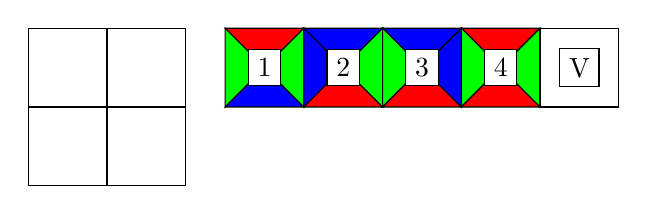
\begin{tikzpicture}

\draw (0,0) grid (2,2);

\draw[fill=red] (0 + 2.5, 0 + 2) -- (0 + 3.5, 0 + 2) -- (0 + 3, 0 + 1.5) -- cycle;
\draw[fill=green] (0 + 2.5, 0 + 2) -- (0 + 2.5, 0 + 1) -- (0 + 3, 0 + 1.5) -- cycle;
\draw[fill=blue] (0 + 2.5, 0 + 1) -- (0 + 3.5, 0 + 1) -- (0 + 3, 0 + 1.5) -- cycle;
\draw[fill=green] (0 + 3.5, 0 + 1) -- (0 + 3.5, 0 + 2) -- (0 + 3, 0 + 1.5) -- cycle;
\node[draw, fill=white] at (0 + 3, 0 + 1.5) {1};

\draw[fill=blue] (1 + 2.5, 0 + 2) -- (1 + 3.5, 0 + 2) -- (1 + 3, 0 + 1.5) -- cycle;
\draw[fill=blue] (1 + 2.5, 0 + 2) -- (1 + 2.5, 0 + 1) -- (1 + 3, 0 + 1.5) -- cycle;
\draw[fill=red] (1 + 2.5, 0 + 1) -- (1 + 3.5, 0 + 1) -- (1 + 3, 0 + 1.5) -- cycle;
\draw[fill=green] (1 + 3.5, 0 + 1) -- (1 + 3.5, 0 + 2) -- (1 + 3, 0 + 1.5) -- cycle;
\node[draw, fill=white] at (1 + 3, 0 + 1.5) {2};

\draw[fill=blue] (2 + 2.5, 0 + 2) -- (2 + 3.5, 0 + 2) -- (2 + 3, 0 + 1.5) -- cycle;
\draw[fill=green] (2 + 2.5, 0 + 2) -- (2 + 2.5, 0 + 1) -- (2 + 3, 0 + 1.5) -- cycle;
\draw[fill=red] (2 + 2.5, 0 + 1) -- (2 + 3.5, 0 + 1) -- (2 + 3, 0 + 1.5) -- cycle;
\draw[fill=blue] (2 + 3.5, 0 + 1) -- (2 + 3.5, 0 + 2) -- (2 + 3, 0 + 1.5) -- cycle;
\node[draw, fill=white] at (2 + 3, 0 + 1.5) {3};

\draw[fill=red] (3 + 2.5, 0 + 2) -- (3 + 3.5, 0 + 2) -- (3 + 3, 0 + 1.5) -- cycle;
\draw[fill=green] (3 + 2.5, 0 + 2) -- (3 + 2.5, 0 + 1) -- (3 + 3, 0 + 1.5) -- cycle;
\draw[fill=red] (3 + 2.5, 0 + 1) -- (3 + 3.5, 0 + 1) -- (3 + 3, 0 + 1.5) -- cycle;
\draw[fill=green] (3 + 3.5, 0 + 1) -- (3 + 3.5, 0 + 2) -- (3 + 3, 0 + 1.5) -- cycle;
\node[draw, fill=white] at (3 + 3, 0 + 1.5) {4};

\draw[black] (4 + 2.5, 0 + 2) rectangle (5 + 2.5, 1);
\node[draw, fill=white] at (4 + 3, 0 + 1.5) {V};

\end{tikzpicture}

\caption{Tablero y fichas de entrada. La ficha \emph{V} va a representar dejar el casillero vac\'io}
\label{ej_3:entrada}
\end{figure}

\begin{figure}[!htbp]
\centering
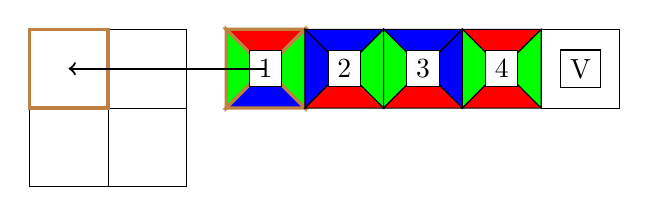
\begin{tikzpicture}

\draw (0,0) grid (2,2);

\draw[brown,very thick] (0,2) rectangle (1,1);

\draw[brown,very thick,fill=red] (0 + 2.5, 0 + 2) -- (0 + 3.5, 0 + 2) -- (0 + 3, 0 + 1.5) -- cycle;
\draw[brown,very thick,fill=green] (0 + 2.5, 0 + 2) -- (0 + 2.5, 0 + 1) -- (0 + 3, 0 + 1.5) -- cycle;
\draw[brown,very thick,fill=blue] (0 + 2.5, 0 + 1) -- (0 + 3.5, 0 + 1) -- (0 + 3, 0 + 1.5) -- cycle;
\draw[brown,very thick,fill=green] (0 + 3.5, 0 + 1) -- (0 + 3.5, 0 + 2) -- (0 + 3, 0 + 1.5) -- cycle;
\node[draw, fill=white] at (0 + 3, 0 + 1.5) {1};

\draw[->,thick] (0 + 3, 0 + 1.5) -- (0 + 0.5, 0 + 1.5);

\draw[fill=blue] (1 + 2.5, 0 + 2) -- (1 + 3.5, 0 + 2) -- (1 + 3, 0 + 1.5) -- cycle;
\draw[fill=blue] (1 + 2.5, 0 + 2) -- (1 + 2.5, 0 + 1) -- (1 + 3, 0 + 1.5) -- cycle;
\draw[fill=red] (1 + 2.5, 0 + 1) -- (1 + 3.5, 0 + 1) -- (1 + 3, 0 + 1.5) -- cycle;
\draw[fill=green] (1 + 3.5, 0 + 1) -- (1 + 3.5, 0 + 2) -- (1 + 3, 0 + 1.5) -- cycle;
\node[draw, fill=white] at (1 + 3, 0 + 1.5) {2};

\draw[fill=blue] (2 + 2.5, 0 + 2) -- (2 + 3.5, 0 + 2) -- (2 + 3, 0 + 1.5) -- cycle;
\draw[fill=green] (2 + 2.5, 0 + 2) -- (2 + 2.5, 0 + 1) -- (2 + 3, 0 + 1.5) -- cycle;
\draw[fill=red] (2 + 2.5, 0 + 1) -- (2 + 3.5, 0 + 1) -- (2 + 3, 0 + 1.5) -- cycle;
\draw[fill=blue] (2 + 3.5, 0 + 1) -- (2 + 3.5, 0 + 2) -- (2 + 3, 0 + 1.5) -- cycle;
\node[draw, fill=white] at (2 + 3, 0 + 1.5) {3};

\draw[fill=red] (3 + 2.5, 0 + 2) -- (3 + 3.5, 0 + 2) -- (3 + 3, 0 + 1.5) -- cycle;
\draw[fill=green] (3 + 2.5, 0 + 2) -- (3 + 2.5, 0 + 1) -- (3 + 3, 0 + 1.5) -- cycle;
\draw[fill=red] (3 + 2.5, 0 + 1) -- (3 + 3.5, 0 + 1) -- (3 + 3, 0 + 1.5) -- cycle;
\draw[fill=green] (3 + 3.5, 0 + 1) -- (3 + 3.5, 0 + 2) -- (3 + 3, 0 + 1.5) -- cycle;
\node[draw, fill=white] at (3 + 3, 0 + 1.5) {4};

\draw[black] (4 + 2.5, 0 + 2) rectangle (5 + 2.5, 1);
\node[draw, fill=white] at (4 + 3, 0 + 1.5) {V};

\end{tikzpicture}

\caption{Comienza con la primer posici\'on del tablero y la primera ficha disponible para colocar, siendo esta v\'alida para ser colocada}
\label{ej_3:primera}
\end{figure}

\begin{figure}[!htbp]
\centering
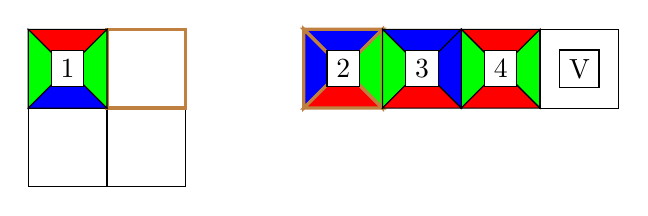
\begin{tikzpicture}

\draw (0,0) grid (2,2);

\draw[brown,very thick] (1,2) rectangle (2,1);

\draw[fill=red] (0 + 0, 0 + 2) -- (0 + 1, 0 + 2) -- (0 + 0.5, 0 + 1.5) -- cycle;
\draw[fill=green] (0 + 0, 0 + 2) -- (0 + 0, 0 + 1) -- (0 + 0.5, 0 + 1.5) -- cycle;
\draw[fill=blue] (0 + 0, 0 + 1) -- (0 + 1, 0 + 1) -- (0 + 0.5, 0 + 1.5) -- cycle;
\draw[fill=green] (0 + 1, 0 + 1) -- (0 + 1, 0 + 2) -- (0 + 0.5, 0 + 1.5) -- cycle;
\node[draw, fill=white] at (0 + 0.5, 0 + 1.5) {1};

\draw[brown,very thick,fill=blue] (1 + 2.5, 0 + 2) -- (1 + 3.5, 0 + 2) -- (1 + 3, 0 + 1.5) -- cycle;
\draw[brown,very thick,fill=blue] (1 + 2.5, 0 + 2) -- (1 + 2.5, 0 + 1) -- (1 + 3, 0 + 1.5) -- cycle;
\draw[brown,very thick,fill=red] (1 + 2.5, 0 + 1) -- (1 + 3.5, 0 + 1) -- (1 + 3, 0 + 1.5) -- cycle;
\draw[brown,very thick,fill=green] (1 + 3.5, 0 + 1) -- (1 + 3.5, 0 + 2) -- (1 + 3, 0 + 1.5) -- cycle;
\node[draw, fill=white] at (1 + 3, 0 + 1.5) {2};

\draw[fill=blue] (2 + 2.5, 0 + 2) -- (2 + 3.5, 0 + 2) -- (2 + 3, 0 + 1.5) -- cycle;
\draw[fill=green] (2 + 2.5, 0 + 2) -- (2 + 2.5, 0 + 1) -- (2 + 3, 0 + 1.5) -- cycle;
\draw[fill=red] (2 + 2.5, 0 + 1) -- (2 + 3.5, 0 + 1) -- (2 + 3, 0 + 1.5) -- cycle;
\draw[fill=blue] (2 + 3.5, 0 + 1) -- (2 + 3.5, 0 + 2) -- (2 + 3, 0 + 1.5) -- cycle;
\node[draw, fill=white] at (2 + 3, 0 + 1.5) {3};

\draw[fill=red] (3 + 2.5, 0 + 2) -- (3 + 3.5, 0 + 2) -- (3 + 3, 0 + 1.5) -- cycle;
\draw[fill=green] (3 + 2.5, 0 + 2) -- (3 + 2.5, 0 + 1) -- (3 + 3, 0 + 1.5) -- cycle;
\draw[fill=red] (3 + 2.5, 0 + 1) -- (3 + 3.5, 0 + 1) -- (3 + 3, 0 + 1.5) -- cycle;
\draw[fill=green] (3 + 3.5, 0 + 1) -- (3 + 3.5, 0 + 2) -- (3 + 3, 0 + 1.5) -- cycle;
\node[draw, fill=white] at (3 + 3, 0 + 1.5) {4};

\draw[black] (4 + 2.5, 0 + 2) rectangle (5 + 2.5, 1);
\node[draw, fill=white] at (4 + 3, 0 + 1.5) {V};

\end{tikzpicture}

\caption{Se mueve a la segunda posici\'on el tablero y analiza la primer ficha disponible, pero no es v\'alida su colocaci\'on}
\label{ej_3:segunda}
\end{figure}

\begin{figure}[!htbp]
\centering
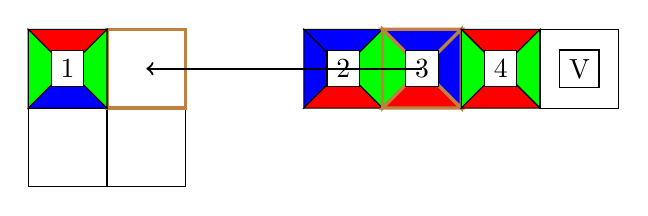
\begin{tikzpicture}

\draw (0,0) grid (2,2);

\draw[brown,very thick] (1,2) rectangle (2,1);

\draw[fill=red] (0 + 0, 0 + 2) -- (0 + 1, 0 + 2) -- (0 + 0.5, 0 + 1.5) -- cycle;
\draw[fill=green] (0 + 0, 0 + 2) -- (0 + 0, 0 + 1) -- (0 + 0.5, 0 + 1.5) -- cycle;
\draw[fill=blue] (0 + 0, 0 + 1) -- (0 + 1, 0 + 1) -- (0 + 0.5, 0 + 1.5) -- cycle;
\draw[fill=green] (0 + 1, 0 + 1) -- (0 + 1, 0 + 2) -- (0 + 0.5, 0 + 1.5) -- cycle;
\node[draw, fill=white] at (0 + 0.5, 0 + 1.5) {1};

\draw[fill=blue] (1 + 2.5, 0 + 2) -- (1 + 3.5, 0 + 2) -- (1 + 3, 0 + 1.5) -- cycle;
\draw[fill=blue] (1 + 2.5, 0 + 2) -- (1 + 2.5, 0 + 1) -- (1 + 3, 0 + 1.5) -- cycle;
\draw[fill=red] (1 + 2.5, 0 + 1) -- (1 + 3.5, 0 + 1) -- (1 + 3, 0 + 1.5) -- cycle;
\draw[fill=green] (1 + 3.5, 0 + 1) -- (1 + 3.5, 0 + 2) -- (1 + 3, 0 + 1.5) -- cycle;
\node[draw, fill=white] at (1 + 3, 0 + 1.5) {2};

\draw[brown,very thick,fill=blue] (2 + 2.5, 0 + 2) -- (2 + 3.5, 0 + 2) -- (2 + 3, 0 + 1.5) -- cycle;
\draw[brown,very thick,fill=green] (2 + 2.5, 0 + 2) -- (2 + 2.5, 0 + 1) -- (2 + 3, 0 + 1.5) -- cycle;
\draw[brown,very thick,fill=red] (2 + 2.5, 0 + 1) -- (2 + 3.5, 0 + 1) -- (2 + 3, 0 + 1.5) -- cycle;
\draw[brown,very thick,fill=blue] (2 + 3.5, 0 + 1) -- (2 + 3.5, 0 + 2) -- (2 + 3, 0 + 1.5) -- cycle;
\node[draw, fill=white] at (2 + 3, 0 + 1.5) {3};

\draw[->,thick] (0 + 5, 0 + 1.5) -- (0 + 1.5, 0 + 1.5);

\draw[fill=red] (3 + 2.5, 0 + 2) -- (3 + 3.5, 0 + 2) -- (3 + 3, 0 + 1.5) -- cycle;
\draw[fill=green] (3 + 2.5, 0 + 2) -- (3 + 2.5, 0 + 1) -- (3 + 3, 0 + 1.5) -- cycle;
\draw[fill=red] (3 + 2.5, 0 + 1) -- (3 + 3.5, 0 + 1) -- (3 + 3, 0 + 1.5) -- cycle;
\draw[fill=green] (3 + 3.5, 0 + 1) -- (3 + 3.5, 0 + 2) -- (3 + 3, 0 + 1.5) -- cycle;
\node[draw, fill=white] at (3 + 3, 0 + 1.5) {4};

\draw[black] (4 + 2.5, 0 + 2) rectangle (5 + 2.5, 1);
\node[draw, fill=white] at (4 + 3, 0 + 1.5) {V};

\end{tikzpicture}

\caption{Ahora analiza la ficha n\'umero 3, la cual si es v\'alida colocar}
\label{ej_3:segunda_valida}
\end{figure}

\begin{figure}[!htbp]
\centering
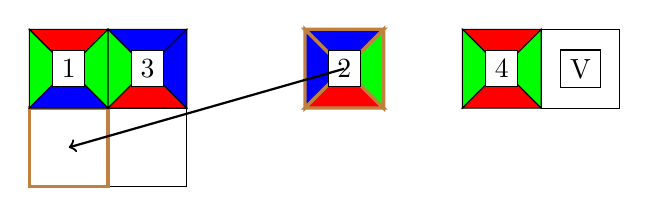
\begin{tikzpicture}

\draw (0,0) grid (2,2);

\draw[brown,very thick] (0,1) rectangle (1,0);

\draw[fill=red] (0 + 0, 0 + 2) -- (0 + 1, 0 + 2) -- (0 + 0.5, 0 + 1.5) -- cycle;
\draw[fill=green] (0 + 0, 0 + 2) -- (0 + 0, 0 + 1) -- (0 + 0.5, 0 + 1.5) -- cycle;
\draw[fill=blue] (0 + 0, 0 + 1) -- (0 + 1, 0 + 1) -- (0 + 0.5, 0 + 1.5) -- cycle;
\draw[fill=green] (0 + 1, 0 + 1) -- (0 + 1, 0 + 2) -- (0 + 0.5, 0 + 1.5) -- cycle;
\node[draw, fill=white] at (0 + 0.5, 1 + 0.5) {1};

\draw[brown,very thick,fill=blue] (1 + 2.5, 0 + 2) -- (1 + 3.5, 0 + 2) -- (1 + 3, 0 + 1.5) -- cycle;
\draw[brown,very thick,fill=blue] (1 + 2.5, 0 + 2) -- (1 + 2.5, 0 + 1) -- (1 + 3, 0 + 1.5) -- cycle;
\draw[brown,very thick,fill=red] (1 + 2.5, 0 + 1) -- (1 + 3.5, 0 + 1) -- (1 + 3, 0 + 1.5) -- cycle;
\draw[brown,very thick,fill=green] (1 + 3.5, 0 + 1) -- (1 + 3.5, 0 + 2) -- (1 + 3, 0 + 1.5) -- cycle;
\node[draw, fill=white] at (1 + 3, 0 + 1.5) {2};

\draw[->,thick] (0 + 4, 0 + 1.5) -- (0 + 0.5, 0 + 0.5);

\draw[fill=blue] (1 + 0, 0 + 2) -- (1 + 1, 0 + 2) -- (1 + 0.5, 0 + 1.5) -- cycle;
\draw[fill=green] (1 + 0, 0 + 2) -- (1 + 0, 0 + 1) -- (1 + 0.5, 0 + 1.5) -- cycle;
\draw[fill=red] (1 + 0, 0 + 1) -- (1 + 1, 0 + 1) -- (1 + 0.5, 0 + 1.5) -- cycle;
\draw[fill=blue] (1 + 1, 0 + 1) -- (1 + 1, 0 + 2) -- (1 + 0.5, 0 + 1.5) -- cycle;
\node[draw, fill=white] at (1 + 0.5, 1 + 0.5) {3};

\draw[fill=red] (3 + 2.5, 0 + 2) -- (3 + 3.5, 0 + 2) -- (3 + 3, 0 + 1.5) -- cycle;
\draw[fill=green] (3 + 2.5, 0 + 2) -- (3 + 2.5, 0 + 1) -- (3 + 3, 0 + 1.5) -- cycle;
\draw[fill=red] (3 + 2.5, 0 + 1) -- (3 + 3.5, 0 + 1) -- (3 + 3, 0 + 1.5) -- cycle;
\draw[fill=green] (3 + 3.5, 0 + 1) -- (3 + 3.5, 0 + 2) -- (3 + 3, 0 + 1.5) -- cycle;
\node[draw, fill=white] at (3 + 3, 0 + 1.5) {4};

\draw[black] (4 + 2.5, 0 + 2) rectangle (5 + 2.5, 1);
\node[draw, fill=white] at (4 + 3, 0 + 1.5) {V};

\end{tikzpicture}

\caption{Avanza al siguiente casillero y vuelve a fijarse en la segunda ficha disponible para poner, como es v\'alida, la coloca}
\label{ej_3:ante_ultima}
\end{figure}

\begin{figure}[!htbp]
\centering
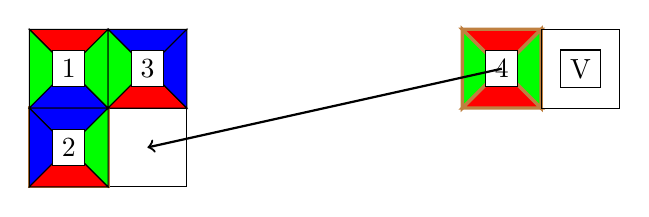
\begin{tikzpicture}

\draw (0,0) grid (2,2);

\draw[brown,very thick] (0,1) rectangle (1,0);

\draw[fill=red] (0 + 0, 0 + 2) -- (0 + 1, 0 + 2) -- (0 + 0.5, 0 + 1.5) -- cycle;
\draw[fill=green] (0 + 0, 0 + 2) -- (0 + 0, 0 + 1) -- (0 + 0.5, 0 + 1.5) -- cycle;
\draw[fill=blue] (0 + 0, 0 + 1) -- (0 + 1, 0 + 1) -- (0 + 0.5, 0 + 1.5) -- cycle;
\draw[fill=green] (0 + 1, 0 + 1) -- (0 + 1, 0 + 2) -- (0 + 0.5, 0 + 1.5) -- cycle;
\node[draw, fill=white] at (0 + 0.5, 1 + 0.5) {1};

\draw[fill=blue] (0 + 0, 0 + 1) -- (0 + 1, 0 + 1) -- (0 + 0.5, 0 + 0.5) -- cycle;
\draw[fill=blue] (0 + 0, 0 + 1) -- (0 + 0, 0 + 0) -- (0 + 0.5, 0 + 0.5) -- cycle;
\draw[fill=red]  (0 + 0, 0 + 0) -- (0 + 1, 0 + 0) -- (0 + 0.5, 0 + 0.5) -- cycle;
\draw[fill=green] (0 + 1, 0 + 0) -- (0 + 1, 0 + 1) -- (0 + 0.5, 0 + 0.5) -- cycle;
\node[draw, fill=white] at (0 + 0.5, 0 + 0.5) {2};

\draw[fill=blue] (1 + 0, 0 + 2) -- (1 + 1, 0 + 2) -- (1 + 0.5, 0 + 1.5) -- cycle;
\draw[fill=green] (1 + 0, 0 + 2) -- (1 + 0, 0 + 1) -- (1 + 0.5, 0 + 1.5) -- cycle;
\draw[fill=red] (1 + 0, 0 + 1) -- (1 + 1, 0 + 1) -- (1 + 0.5, 0 + 1.5) -- cycle;
\draw[fill=blue] (1 + 1, 0 + 1) -- (1 + 1, 0 + 2) -- (1 + 0.5, 0 + 1.5) -- cycle;
\node[draw, fill=white] at (1 + 0.5, 1 + 0.5) {3};

\draw[brown,very thick,fill=red] (3 + 2.5, 0 + 2) -- (3 + 3.5, 0 + 2) -- (3 + 3, 0 + 1.5) -- cycle;
\draw[brown,very thick,fill=green] (3 + 2.5, 0 + 2) -- (3 + 2.5, 0 + 1) -- (3 + 3, 0 + 1.5) -- cycle;
\draw[brown,very thick,fill=red] (3 + 2.5, 0 + 1) -- (3 + 3.5, 0 + 1) -- (3 + 3, 0 + 1.5) -- cycle;
\draw[brown,very thick,fill=green] (3 + 3.5, 0 + 1) -- (3 + 3.5, 0 + 2) -- (3 + 3, 0 + 1.5) -- cycle;
\node[draw, fill=white] at (3 + 3, 0 + 1.5) {4};

\draw[->,thick] (0 + 6, 0 + 1.5) -- (0 + 1.5, 0 + 0.5);

\draw[black] (4 + 2.5, 0 + 2) rectangle (5 + 2.5, 1);
\node[draw, fill=white] at (4 + 3, 0 + 1.5) {V};

\end{tikzpicture}

\caption{Avanza al \'ultimo casillero y se fija en la \'ultima ficha disponible que queda, como es v\'alida, la coloca}
\label{ej_3:ultima_ficha}
\end{figure}

\begin{figure}[!htbp]
\centering
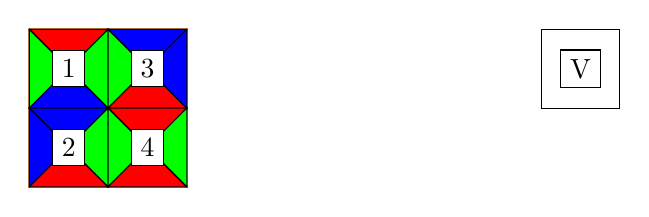
\begin{tikzpicture}

\draw[brown,very thick] (0,0) grid (2,2);

\draw[fill=red] (0 + 0, 0 + 2) -- (0 + 1, 0 + 2) -- (0 + 0.5, 0 + 1.5) -- cycle;
\draw[fill=green] (0 + 0, 0 + 2) -- (0 + 0, 0 + 1) -- (0 + 0.5, 0 + 1.5) -- cycle;
\draw[fill=blue] (0 + 0, 0 + 1) -- (0 + 1, 0 + 1) -- (0 + 0.5, 0 + 1.5) -- cycle;
\draw[fill=green] (0 + 1, 0 + 1) -- (0 + 1, 0 + 2) -- (0 + 0.5, 0 + 1.5) -- cycle;
\node[draw, fill=white] at (0 + 0.5, 1 + 0.5) {1};

\draw[fill=blue] (0 + 0, 0 + 1) -- (0 + 1, 0 + 1) -- (0 + 0.5, 0 + 0.5) -- cycle;
\draw[fill=blue] (0 + 0, 0 + 1) -- (0 + 0, 0 + 0) -- (0 + 0.5, 0 + 0.5) -- cycle;
\draw[fill=red]  (0 + 0, 0 + 0) -- (0 + 1, 0 + 0) -- (0 + 0.5, 0 + 0.5) -- cycle;
\draw[fill=green] (0 + 1, 0 + 0) -- (0 + 1, 0 + 1) -- (0 + 0.5, 0 + 0.5) -- cycle;
\node[draw, fill=white] at (0 + 0.5, 0 + 0.5) {2};

\draw[fill=blue] (1 + 0, 0 + 2) -- (1 + 1, 0 + 2) -- (1 + 0.5, 0 + 1.5) -- cycle;
\draw[fill=green] (1 + 0, 0 + 2) -- (1 + 0, 0 + 1) -- (1 + 0.5, 0 + 1.5) -- cycle;
\draw[fill=red] (1 + 0, 0 + 1) -- (1 + 1, 0 + 1) -- (1 + 0.5, 0 + 1.5) -- cycle;
\draw[fill=blue] (1 + 1, 0 + 1) -- (1 + 1, 0 + 2) -- (1 + 0.5, 0 + 1.5) -- cycle;
\node[draw, fill=white] at (1 + 0.5, 1 + 0.5) {3};

\draw[fill=red]  (1 + 0, 0 + 1) -- (1 + 1, 0 + 1) -- (1 + 0.5, 0 + 0.5) -- cycle;
\draw[fill=green] (1 + 0, 0 + 1) -- (1 + 0, 0 + 0) -- (1 + 0.5, 0 + 0.5) -- cycle;
\draw[fill=red] (1 + 0, 0 + 0) -- (1 + 1, 0 + 0) -- (1 + 0.5, 0 + 0.5) -- cycle;
\draw[fill=green] (1 + 1, 0 + 0) -- (1 + 1, 0 + 1) -- (1 + 0.5, 0 + 0.5) -- cycle;
\node[draw, fill=white] at (1 + 0.5, 0 + 0.5) {4};

\draw[black] (4 + 2.5, 0 + 2) rectangle (5 + 2.5, 1);
\node[draw, fill=white] at (4 + 3, 0 + 1.5) {V};

\end{tikzpicture}

\caption{Al no quedar casillero sin procesar, se llega al caso base y guarda la combinaci\'on como la m\'axima encontrada}
\label{ej_3:caso_base}
\end{figure}

\begin{figure}[!htbp]
\centering
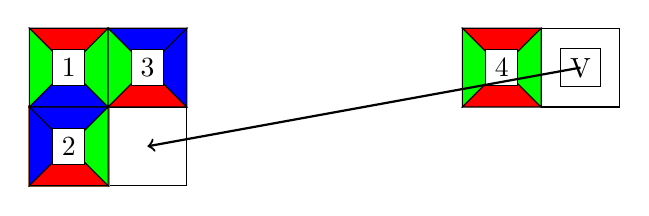
\begin{tikzpicture}

\draw (0,0) grid (2,2);

\draw[brown,very thick] (0,1) rectangle (1,0);

\draw[fill=red] (0 + 0, 0 + 2) -- (0 + 1, 0 + 2) -- (0 + 0.5, 0 + 1.5) -- cycle;
\draw[fill=green] (0 + 0, 0 + 2) -- (0 + 0, 0 + 1) -- (0 + 0.5, 0 + 1.5) -- cycle;
\draw[fill=blue] (0 + 0, 0 + 1) -- (0 + 1, 0 + 1) -- (0 + 0.5, 0 + 1.5) -- cycle;
\draw[fill=green] (0 + 1, 0 + 1) -- (0 + 1, 0 + 2) -- (0 + 0.5, 0 + 1.5) -- cycle;
\node[draw, fill=white] at (0 + 0.5, 1 + 0.5) {1};

\draw[fill=blue] (0 + 0, 0 + 1) -- (0 + 1, 0 + 1) -- (0 + 0.5, 0 + 0.5) -- cycle;
\draw[fill=blue] (0 + 0, 0 + 1) -- (0 + 0, 0 + 0) -- (0 + 0.5, 0 + 0.5) -- cycle;
\draw[fill=red]  (0 + 0, 0 + 0) -- (0 + 1, 0 + 0) -- (0 + 0.5, 0 + 0.5) -- cycle;
\draw[fill=green] (0 + 1, 0 + 0) -- (0 + 1, 0 + 1) -- (0 + 0.5, 0 + 0.5) -- cycle;
\node[draw, fill=white] at (0 + 0.5, 0 + 0.5) {2};

\draw[fill=blue] (1 + 0, 0 + 2) -- (1 + 1, 0 + 2) -- (1 + 0.5, 0 + 1.5) -- cycle;
\draw[fill=green] (1 + 0, 0 + 2) -- (1 + 0, 0 + 1) -- (1 + 0.5, 0 + 1.5) -- cycle;
\draw[fill=red] (1 + 0, 0 + 1) -- (1 + 1, 0 + 1) -- (1 + 0.5, 0 + 1.5) -- cycle;
\draw[fill=blue] (1 + 1, 0 + 1) -- (1 + 1, 0 + 2) -- (1 + 0.5, 0 + 1.5) -- cycle;
\node[draw, fill=white] at (1 + 0.5, 1 + 0.5) {3};

\draw[fill=red] (3 + 2.5, 0 + 2) -- (3 + 3.5, 0 + 2) -- (3 + 3, 0 + 1.5) -- cycle;
\draw[fill=green] (3 + 2.5, 0 + 2) -- (3 + 2.5, 0 + 1) -- (3 + 3, 0 + 1.5) -- cycle;
\draw[fill=red] (3 + 2.5, 0 + 1) -- (3 + 3.5, 0 + 1) -- (3 + 3, 0 + 1.5) -- cycle;
\draw[fill=green] (3 + 3.5, 0 + 1) -- (3 + 3.5, 0 + 2) -- (3 + 3, 0 + 1.5) -- cycle;
\node[draw, fill=white] at (3 + 3, 0 + 1.5) {4};


\draw[black] (4 + 2.5, 0 + 2) rectangle (5 + 2.5, 1);
\node[draw, fill=white] at (4 + 3, 0 + 1.5) {V};

\draw[->,thick] (0 + 7, 0 + 1.5) -- (1 + 0.5, 0 + 0.5);

\end{tikzpicture}

\caption{Habiendo retornado de la recursi\'on y volviendo al paso de la imagen \ref{ej_3:ultima_ficha}, la ficha que queda por colocar es la que representa al casillero vac\'io}
\label{ej_3:ficha_vacia}
\end{figure}



\newpage

\subsection{Correctitud} \label{ej_3:justificacion}

Como se coment\'o en la secci\'on de la idea de la resoluci\'on (\ref{ej_3:idea}), tenemos $\sum_{i=0}^{k}\binom{k}{i}\frac{k!}{i!} \label{ej_3:k}$ (\ref{ej_3:combinaciones}) combinaciones diferentes del cubo, si el algoritmo las recorre todas y toma la m\'axima combinaci\'on v\'alida,
entonces el algoritmo es correcto, ya que no le quedar\'ia ninguna combinaci\'on por validar.
Pero el algoritmo no chequea todas las combinaciones, la idea es descartar las combinaciones en las que las fichas no est\'an colocadas correctamente, y realiza una \emph{poda}, por lo que hay que justificar si el algoritmo saca el m\'aximo de un conjunto de soluciones posibles correctamente, y si dicho conjunto de posibles soluciones compuesto por todas las posibles combinaciones descartando las que contienen fichas adyacentes que no tienen el mismo color y quitando los que descarta la poda, contiene la soluci\'on m\'axima que se est\'a buscando.

Sin la l\'inea \ref{ej_3:pseudo:valida} del algoritmo (\ref{ej_3:pseudo}) que valida la ficha a colocar, el algoritmo recorre todas las posiciones y en cada una recorre todas las fichas disponibles, y s\'olo saca la ficha de disponibildiad cuando la coloca, es decir, si una ficha no est\'a disponible es porque ya fue colocada y las fichas no se pueden repetir.

En el descarte de las combinaciones que las fichas no est\'an colocadas correctamente, la soluci\'on que se pide encontrar tiene que contener todas las fichas colocadas correctamente, tal que 2 fichas adyacentes tengan el lado en com\'un con el mismo color, por lo que descartar las combinaciones no v\'alidas no est\'a descartando la soluci\'on que se pide encontrar.
El algoritmo (\ref{ej_3:pseudo}) recorre el tablero de izquierda a derecha y de arriba a abajo, y en cada posici\'on recorre todas las fichas disponibles, la coloca si es v\'alida, y contin\'ua a la siguiente posici\'on quitando como disponible la ficha colocada, cuando retorna de la recursi\'on, la ficha que se hab\'ia colocado se vuelve a poner como disponible y contin\'ua con la pr\'oxima ficha disponible. Si la ficha no es v\'alida, entonces descarta todas las combinaciones que comienzen con las fichas:
\begin{equation}
	\{f_0,\dotsc,f_i\}
\end{equation}
siendo $f_i$ la ficha no v\'alida de colocar, y $\{f_0,\dotsc,f_{i-1}\}$ las fichas colocadas en los pasos anteriores, y como todas las fichas en la soluci\'on que se quiere encontrar tienen que estar puestas correctamente, entonces \'esta soluci\'on no puede comenzar con $\{f_0,\dotsc,f_i\}$ por tener una ficha que no es v\'alida de colocar en esa posici\'on

En el caso de la \emph{poda}, el algoritmo tiene la variable $fichas\_maximas$ que contiene la cantidad m\'axima de fichas que se pudieron colocar (y se tiene dicha combinaci\'on almacenada), la condici\'on de la \emph{poda} es (l\'inea \ref{ej_3:pseudo:poda} del algoritmo \ref{ej_3:pseudo})
\begin{algorithmic}
	\If{$total\_casilleros - casilleros\_calculados + fichas\_colocadas <= fichas\_maxima$}
		\State return
	\EndIf
\end{algorithmic}
Siendo $total\_casilleros$ los casilleros del tablero, $casilleros\_calculados$ la cantidad de casilleros que ya se colocaron fichas o se dejaron vac\'io, y $fichas\_colocadas$ la cantidad de casilleros con fichas hasta el momento. Si dicha condici\'on se cumple, entonces corta con la recursi\'on y no contin\'ua intentando.
Lo que se quiere encontrar es para todos los tableros, obtener el que tiene mas fichas colocadas.
\begin{equation}
	\forall (tablero) fichas\_colocadas(tablero\_optimo) >= fichas\_colocadas(tablero)
\end{equation}
Para el tablero en particular en construcci\'on que se est\'a armando, los casilleros restantes por calcular son $total\_casilleros - casilleros\_calculados$, como buscamos el tablero con mayor cantidad de fichas, lo mejor que podemos obtener de un tablero en particular en construcci\'on es que la totalidad de casilleros restantes contengan fichas, en ese caso a la cantidad de fichas ya colocadas, le sumamos los casilleros restantes
\begin{equation}
	total\_casilleros - casilleros\_calculados + fichas\_colocadas
\end{equation}
Si $fichas\_maximas >= total\_casilleros - casilleros\_calculados + fichas\_colocadas$, este tablero en construcci\'on tendr\'a menor o igual de fichas que $fichas\_maximas$ porque para tener m\'as fichas tendr\'ia que tener m\'as casilleros, y como s\'olo nos interesa 1 soluci\'on, si es igual la podemos descartar una vez ya se encontr\'o una. Entonces, la \emph{poda} descarta combinaciones que son menores o iguales que el m\'aximo, ya que si el m\'aximo es el que est\'a en $tablero\_optimo$,
descarta combinaciones con igual o menor cantidad de fichas, y si el m\'aximo es otro aun no encontrado, entonces va a tener m\'as fichas que $tablero\_optimo$ y m\'as que que tablero en construcci\'on (\ref{ej_3:no_encontrada}), por lo que el tablero en construcci\'on tampoco es soluci\'on
\begin{equation}
\begin{split}
	solucion\_aun\_no\_encontrada > fichas\_maximas >=\\
	total\_casilleros - casilleros\_calculados + fichas\_colocadas \label{ej_3:no_encontrada}
\end{split}
\end{equation}

Sabiendo que las combinaciones que se descartan no son soluciones correctas, el algoritmo para guardar el m\'aximo realiza lo siguiente una vez que no quedan casilleros por procesar:
\begin{algorithmic}
	\If{$fichas\_colocadas > fichas\_maximas$}
		\State copiarTablero(tablero\_optimo, tablero)
		\State $fichas\_maximas \gets fichas\_colocadas$
	\EndIf
\end{algorithmic}
Y por cada ficha que se coloca, realiza:
\begin{algorithmic}
	\If{$\neg f->vacia$}
		\State $fichas\_nuevas \gets fichas\_disponibles - f$
		\State $fichas\_colocadas++$
	\Else
		\State $fichas\_nuevas \gets fichas\_disponibles$
	\EndIf
	\State maximizarTablero(tablero, n, m, fichas\_nuevas, i\_proximo, j\_proximo, casilleros\_calculados + 1, fichas\_colocadas, tablero\_optimo, fichas\_maximas)
\end{algorithmic}
Por cada ficha que no sea dejar el casillero vac\'io, se incrementa la cantidad de fichas colocadas y se le pasa recursivamente a la funci\'on, si la llamada recursiva llega al caso base, $fichas\_colocadas$ tendr\'a la cantidad de fichas puestas,
y por la condici\'on $fichas\_colocadas > fichas\_maximas$, si se cumple significa que se encontr\'o un tablero con m\'as fichas, y se guarda en $tablero\_optimo$ y en $fichas\_maximas$ los valores correspondientes. Como se llama a la funci\'on con el valor $fichas\_maximas < 0$ (como est\'a explicado en la secci\'on \ref{ej_3:algo}), entonces con el primer tablero que calcule aunque sea dejar todo vac\'io obteniendo la cantidad m\'inima de fichas colocadas ($0$), ya va a cumlir que es mayor a $fichas\_maximas$ y va a colocar el tablero como posible soluci\'on.

Entonces, se vi\'o que los casos que descarta no contienen a la soluci\'on o bien tienen la misma cantidad de fichas que alguna la soluci\'on encontrada, y el algoritmo siempre se queda con el m\'aximo encontrado hasta el momento.

Como se recorre primero por columnas de izquierda a derecha y luego por filas de arriba a abajo, las fichas a colocar s\'olo pueden ser validadas contra 2 bordes de sus fichas adyacentes, arriba y/o izquierda, ya que no hay fichas a\'un colocadas a la derecha y abajo porque a\'un no se procesaron esos casilleros, si la ficha a colocar est\'a en la primera fila, no hay que verificar el color de arriba, y si est\'a en la primer columna, no hay que verificar el color izquierda. El tablero comienza vac\'io por lo que cada ficha que se coloca es validad, y al colocar una ficha, todas las anteriores est\'an colocadas correctamente porque ya fueron validadas. 

\subsection{Cota de complejidad} \label{ej_3:cota}

El algoritmo es recursivo y contiene un ciclo donde recorre todas las fichas disponibles (lo implementamos en una lista, y es $O(1)$), y en cada ciclo chequea que la ficha sea v\'alida ($O(1)$) de colocar y se llama recursivamente a la funci\'on, si no se dej\'o el casillero vac\'io entonces hay una ficha menos a recorrer en el ciclo de la llamada recursiva, por lo que nos queda que realiza:
\begin{equation}
\begin{split}
n*m(n*m+1-j_1)(n*m+1-j_2)(\dotsc)(n*m+1-j_{n*m})\\ 
= \prod_{i=0}^{n*m} \left(n*m + 1 - j_i \right)
\end{split}
\end{equation}
Siendo $j_i$ la cantidad de fichas colocadas en el paso $i$ de la recursi\'on ($j_0 = 0$ porque es el primer paso y no se proceso\'o ning\'un casillero a\'un), y a las filas y columnas $n$ $m$ se le suma 1 para contar dejar el casillero vac\'i. Pero para cada $i$, puede variar el valor de $j_i$, ya que si se est\'a procesando el casillero $i$, se pudo haber llegado dejandose diferente cantidad de casilleros vac\'ios anteriormente, pero podemos calcular el peor caso dejar todos los casilleros vac\'ios siempre $(\forall i \in [1;n*m]) j_i = 0$, maximizando el producto, o el mejor caso minimizando el producto, donde siempre se colocaron todas las fichas anteriores $(\forall i \in [1;n*m]) j_i = i - 1$

Cuando encuentra un tablero que puede ser soluci\'on y realiza la copia, como se implementa en una matriz y se copian todos los valores, nos queda $O(n*m)$, lo cu\'al se realiza al llegar al final,
pero por la condici\'on de que se copia si supera la cantidad de fichas que se tienen guardadas (si es igual o menor no copia), entonces nos queda que como m\'aximo va a copiarlo $n*m$ veces (que ser\'ia ir mejorando siempre la soluci\'on agregando 1 ficha), lo que nos queda $O((n*m)^2)$ y lo podemos sacar afuera como una suma aparte de toda la llamda recursiva. Si queremos ver la mayor cantidad de iteraciones, ser\'ia que se est\'en comparando todos las fichas contra todas, quedandonos
\begin{equation}
\begin{split}
	\prod_{i=0}^{n*m} \left(n*m + 1 - j_i \right) + (n*m)^2 \\
	\prod_{i=0}^{n*m} (n*m + 1) + (n*m)^2 \\
	(n*m + 1)^{n*m} + (n*m)^2
\end{split}
\end{equation}
Quedando una complejidad de:
\begin{equation}
	O((n*m)^{n*m}) \label{ej_3:peor_complejidad}
\end{equation}

Tambi\'en podemos calcular que pasar\'ia si logra colocar todas las fichas en la primera iteraci\'on del ciclo sobre las fichas disponibles, qued\'andonos un tablero con la m\'axima cantidad de fichas colocadas en $n*m$ llamadas recursivas, y ahora la poda cortar\'a el resto de las recursiones, aunque en cada retorno de la recursi\'on, se sigue intentando con todas las fichas que quedaban, pero no se ejecutan m\'as recurciones por la poda, quedando

\begin{equation*}
	\sum_{i=1}^{n*m} 1 + \sum_{i=1}^{n*m}i + (n*m)
\end{equation*}
La primer sumatoria es el ingreso a la recursi\'on encontrando una ficha v\'alida en la primera iteraci\'on sobre las fichas disponibles, y la segunda es la vuelta de la recursi\'on, que en la `vuelta' contin\'ua iterando las fichas que faltaban, y como en cada llamda se va quitando la ficha que se coloca, la iteraci\'on en cada llamada es sobre 1 ficha menos. Y por \'ultimo el $n*m$ es la copia de la combinaci\'on m\'axima encontrada, quedandonos entonces
\begin{equation*}
	O(n*m) + O(\sum_{i=1}^{n*m}i) + O(n*m)
\end{equation*}
\begin{equation*}
	O(n*m) + O\left(\frac{n*m(n*m - 1)}{2}\right) + O(n*m)
\end{equation*}
\begin{equation}
	O\left((n*m)^2\right) \label{ej_3:mejor_caso}
\end{equation}

Entonces nos queda que el mejor caso es de complejidad cuadr\'atica sobre la cantidad de casilleros del tablero (\ref{ej_3:mejor_caso}) y el peor caso por acotado por $O(n*m)^{n*m}$ (\ref{ej_3:peor_complejidad})

\subsection{Comentarios y conclusiones}

Dada la complejidad calculada (\ref{ej_3:cota}), las mediciones realizadas (\ref{mediciones_3}) y el c\'alculo de la cantidad de combinaciones posibles (\ref{ej_3:combinaciones}), que la cantidad de operaciones que se realizan para chequear la gran cantidad de combinaciones es muy grande,
aunque realizando la \emph{poda} y descartando las combinaciones que no son v\'alidas puede bajar considerablemente la cantidad de operaciones con determinadas entradas.

Se puede concluir que es un problema complejo que a no ser que se realize otro m\'etodo en vez de buscar todas las posibilidades y sacar el m\'aximo, con problemas de entrada peque\~na, como puede ser un tablero de 5x5 (25 fichas), nos da que tendr\'iamos un m\'aximo de 29533262279404214911002168626 posibilidades para analizar y sacar el m\'aximo.

